\paragraph*{Illustration: Gene/Protein regulatory network inference.}
As an illustration, we applied our sparse multi-attribute GGM approach
to  the NCI-60  cancer  line  data set.   This  data  set consists  in
molecular  profiles  on  a  panel  of 60  diverse  human  cancer  cell
lines. We  use both protein  and gene profiling experiments.   For the
former, we  have  samples for  92 antibodies  from reverse-phase
lysate arrays (RPLA); for the latter, expression is measured for 9,000
RNA with Human Genome U95 affymetrix.  A \emph{consensus set} composed
of 91  protein and the  corresponding gene profiles is  retained for
the $n=60$ samples.

We infer  a sparse  GGM on  each attribute  (gene and  protein), 
separately to start with, and then on its multi-attribute version.  We do this on a large
grid  of the  tuning parameter  and thus  have  three families  of
networks    indexed    by    their   number    of    edges.     Figure
\ref{fig:net_jaccard}  demonstrates  that our  sparse  multi-attribute
method capture the characteristics of both univariate networks, as the
Jaccard similarity  index is  high between each  uni-attribute network
and the multi-attribute  network, while it remains  low when comparing
uni-attribute  networks  together.  This  tends  to  prove  that  this
multi-attribute   version  proposes   a   consensus   version  of   the
interactions at hand in the cell, and one which is hopefully more robust to noise and
small misregulations.
\begin{figure}[htbp!]
  \centering
  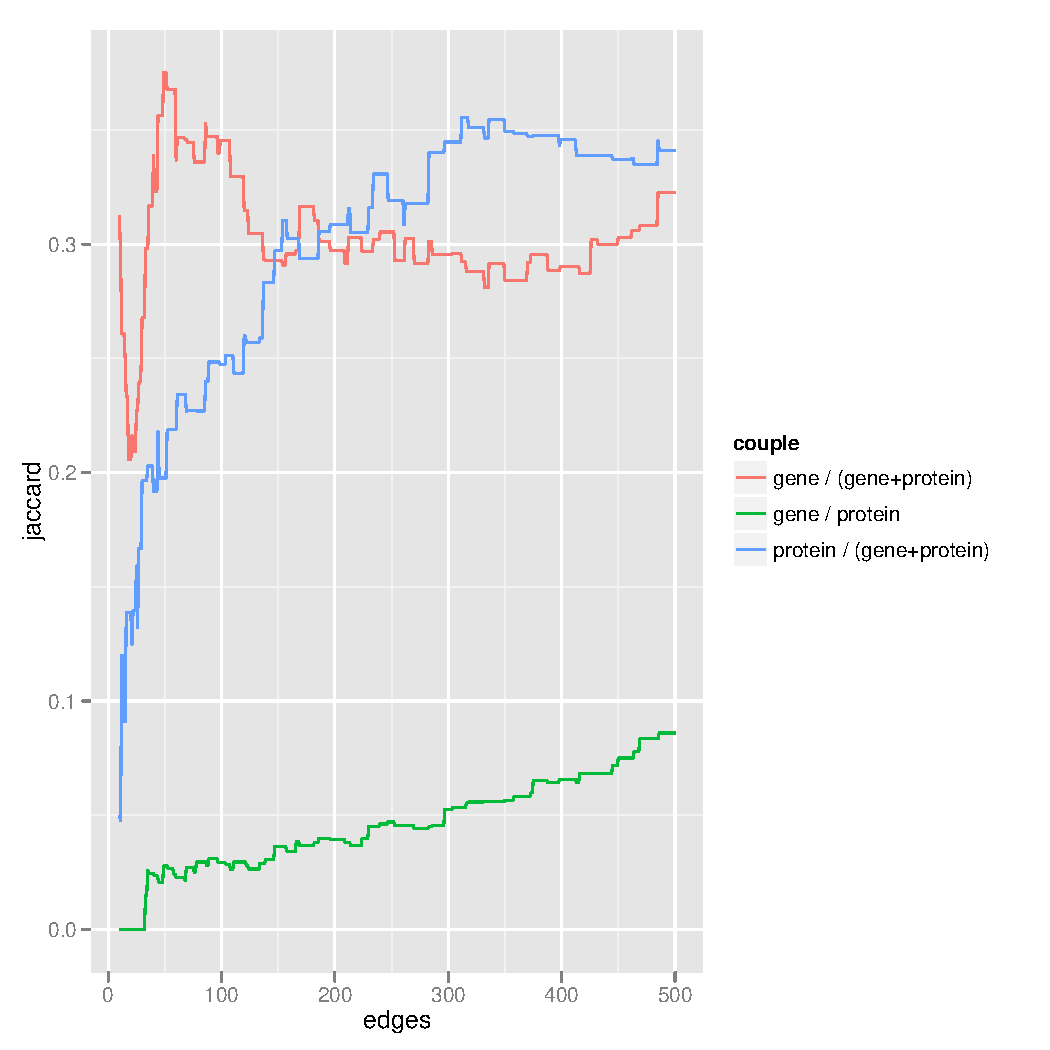
\includegraphics[width=.9\textwidth]{figures/net_jaccard}
  \caption{Jaccard's  similarity index  $J(A,B) =  \frac{\left|A\cap
        B\right|}{\left|A\cup  B\right|}$:  multi-attribute  network
    shares a high Jaccard index with both uni-attribute networks.}
  \label{fig:net_jaccard}
\end{figure}
